% This is the Reed College LaTeX thesis template. Most of the work 
% for the document class was done by Sam Noble (SN), as well as this
% template. Later comments etc. by Ben Salzberg (BTS). Additional
% restructuring and APA support by Jess Youngberg (JY).
% Your comments and suggestions are more than welcome; please email
% them to cus@reed.edu
%
% See http://web.reed.edu/cis/help/latex.html for help. There are a 
% great bunch of help pages there, with notes on
% getting started, bibtex, etc. Go there and read it if you're not
% already familiar with LaTeX.
%
% Any line that starts with a percent symbol is a comment. 
% They won't show up in the document, and are useful for notes 
% to yourself and explaining commands. 
% Commenting also removes a line from the document; 
% very handy for troubleshooting problems. -BTS

% As far as I know, this follows the requirements laid out in 
% the 2002-2003 Senior Handbook. Ask a librarian to check the 
% document before binding. -SN

%%
%% Preamble
%%
% \documentclass{<something>} must begin each LaTeX document
\documentclass[12pt,twoside]{reedthesis}
% Packages are extensions to the basic LaTeX functions. Whatever you
% want to typeset, there is probably a package out there for it.
% Chemistry (chemtex), screenplays, you name it.
% Check out CTAN to see: http://www.ctan.org/
%%
\usepackage{graphicx,latexsym} 
\usepackage{amssymb,amsthm,amsmath}
\usepackage{longtable,booktabs,setspace} 
\usepackage{chemarr} %% Useful for one reaction arrow, useless if you're not a chem major
\usepackage[hyphens]{url}
\usepackage{rotating}
\usepackage{natbib}

\usepackage{tikz}
\usetikzlibrary{arrows}
% Comment out the natbib line above and uncomment the following two lines to use the new 
% biblatex-chicago style, for Chicago A. Also make some changes at the end where the 
% bibliography is included. 
%\usepackage{biblatex-chicago}
%\bibliography{thesis}

% \usepackage{times} % other fonts are available like times, bookman, charter, palatino

\title{To Bayes or Not To Bayes: Bayesian Reasoning About Bayesian Network Structure}
\author{Brett T. Beutell}
% The month and year that you submit your FINAL draft TO THE LIBRARY (May or December)
\date{May 2014}
\division{Mathematics and Natural Sciences}
\advisor{Irena Swanson}
%If you have two advisors for some reason, you can use the following
%\altadvisor{Your Other Advisor}
%%% Remember to use the correct department!
\department{Mathematics}
% if you're writing a thesis in an interdisciplinary major,
% uncomment the line below and change the text as appropriate.
% check the Senior Handbook if unsure.
%\thedivisionof{The Established Interdisciplinary Committee for}
% if you want the approval page to say "Approved for the Committee",
% uncomment the next line
%\approvedforthe{Committee}

\setlength{\parskip}{0pt}

% From example.net/tikz/examples/red-black-tree
\tikzset{
  treenode/.style = {align=center, inner sep=0pt, text centered,
    font=\sffamily},
  arn_n/.style = {treenode, circle, white, font=\sffamily\bfseries, draw=black,
    fill=black, text width=1.5em},% arbre rouge noir, noeud noir
  arn_r/.style = {treenode, circle, red, draw=red, 
    text width=1.5em, very thick},% arbre rouge noir, noeud rouge
  arn_x/.style = {treenode, rectangle, draw=black,
    minimum width=0.5em, minimum height=0.5em}% arbre rouge noir, nil
}

\setcitestyle{square}
%%
%% End Preamble
%%
%% The fun begins:
\begin{document}

  \maketitle
  \frontmatter % this stuff will be roman-numbered
  \pagestyle{empty} % this removes page numbers from the frontmatter

% Acknowledgements (Acceptable American spelling) are optional
% So are Acknowledgments (proper English spelling)
    \chapter*{Acknowledgements}
	I want to thank a few people.

% The preface is optional
% To remove it, comment it out or delete it.
 %   \chapter*{Preface}
%	This is an example of a thesis setup to use the reed thesis document class.

    \tableofcontents
% if you want a list of tables, optional
 %   \listoftables
% if you want a list of figures, also optional
  %  \listoffigures

% The abstract is not required if you're writing a creative thesis (but aren't they all?)
% If your abstract is longer than a page, there may be a formatting issue.
    \chapter*{Abstract}
	Implementing a Bayesian classifier requires finding a suitable network structure and corresponding set of parameters given a set of pre-classified training data. For the most part, estimating the parameters is relatively straightforward, but the space of possible network structures is super-exponential on the number of variables in the model. We explore the use of Markov chain Monte Carlo to simulate draws from the posterior distribution of Bayesian networks given the training data.
	
	\chapter*{Dedication}
	This one's for my parents.

  \mainmatter % here the regular arabic numbering starts
  \pagestyle{fancyplain} % turns page numbering back on

%The \introduction command is provided as a convenience.
%if you want special chapter formatting, you'll probably want to avoid using it altogether

    \chapter*{Introduction}
         \addcontentsline{toc}{chapter}{Introduction}
	\chaptermark{Introduction}
	\markboth{Introduction}{Introduction}
	% The three lines above are to make sure that the headers are right, that the intro gets included in the table of contents, and that it doesn't get numbered 1 so that chapter one is 1.

% Double spacing: if you want to double space, or one and a half 
% space, uncomment one of the following lines. You can go back to 
% single spacing with the \singlespacing command.
% \onehalfspacing
% \doublespacing
	If it were not for convention, this introduction could perhaps be titled, ``An Irresponsibly Quick Introduction to Bayes' Theorem." In the following sections, we introduce the ideas, terminology, and some historical minutiae about Bayesian reasoning. Naturally, we provide a statement of Bayes' theorem for events and distributions.
	\section{Much Ado About Bayes}
	At its inception, Bayes' theorem was not particularly controversial. Pierre Simon Laplace offered its first formalization in the early nineteenth century, and he believed (incorrectly, as was proven by the mid-twentieth century) that with a sufficiently large amount of data, the answers it provided were equivalent to those obtained from his frequency based methods [McGrayne, 2011]. 
	As time passed, Laplace preferred his frequentist techniques for the relative ease of their calculations, but he did not outright condemn the use of Bayes in practice. Interestingly, over a half-century after his death, Laplace's failure to disown Bayesian reasoning caught the attention of Scottish mathematician George Chrystal, who advocated the removal of Bayes' theorem from all academic texts on statistics. He quipped, ``The indiscretions of great men should be quietly allowed to be forgotten" [McGrayne, 2011].
	
	Chrystal's comment represents the mindset of many early twentieth century statisticians. At the time, frequentism reigned supreme, and the attitude towards Bayes' theorem and its role in statistics was surprisingly sour. For years, statisticians in the academy who employed Bayesian reasoning feared for their reputation if they explicitly made reference to Bayes' theorem in their work [McGrayne, 2011]. 
	
	Fortunately, with due thanks to the computational advances of the past three decades, Bayes survived its temporary relegation to the catacombs of statistics, and it has emerged as an astoundingly useful tool for the modern statistician. The phrase ``Bayesian Inference" fails to evoke the contention it once did. Furthermore, it is now far more commonplace for statisticians to use both Bayesian and frequentist techniques in their work, tailoring their methods to the problem at hand [Liu et al, 2013].
	
	Summarily, the use of Bayesian reasoning is no longer divisive or taboo, and it is a recent phenomenon that we may begin our inquiry without several pages apologizing for our inferential philosophy. With that said, it does not hurt to quickly consider the differences between a Bayesian and a frequentist. 
		
\section{To Bayes or Not to Bayes}

	Suppose we seek an estimate of a parameter over some set of random variables. We may call said parameter $\theta$ and our random variables (or, {\em data}) $\vec{X}$. We use $\vec{X}$ to talk about our data in the abstract (that is, before they are observed), and we denote a particular set of observed values as $\vec{x}$. 

	We represent the conditional probability of $\theta$ given a set of observed data as $P(\theta | \vec{X} = \vec{x})$. Vice versa, the conditional probability of the data given a fixed $\theta = \theta_0$ can be written $P(\vec{X} | \theta = \theta_0)$. Note that for the former conditional distribution, we are fixing our data and considering $\theta$ a random variable, whereas for the latter, we are doing the converse.

	\subsection*{``To Bayes"}
	Bayesians prefer the former conditional PDF. To a Bayesian, $\theta$ is uncertain, so the best means of knowing more about $\theta$ is directly through the data. Notably, the choice of words here contains an important qualifier; Bayesians want to know ``{\em more}" about $\theta$. Hence, they specify what is already known about the parameter. Similar to the way mathematicians or logicians use axioms, Bayesians find it important to represent in their methods what it is that they already presume to be true.
	
	We can think of a Bayesian model's presumed truths (often called {\em prior beliefs}, the {\em prior distribution} or, simply, the {\em prior}) as a starting point, from which data are used to {\em update} the subjective belief about the estimate.  Bayesians use what are called {\em non-informative priors} to approximate a lack of prior knowledge about $\theta$. 
	
	Besides the inherent subjectivity of the prior, the essential characteristic of Bayesian methods is that they treat parameters as random variables. Consequently, Bayesian estimates return a probability distribution for $\theta$, which is called the {\em posterior distribution} of $\theta$. The posterior describes the relative likelihoods of different values of $\theta$ given the data and given the {\em a priori} beliefs encoded in the prior distribution.

	\subsection*{``Not To Bayes"}
	For the student of frequentism, the Bayesian approach may lend itself to confusion (or, years ago, anger), since frequentists prefer to think of how probable their observed data are given a fixed $\theta = \theta_0$.
	
	Frequentist techniques have two main advantages. Namely, the math involved in their calculations is generally tidy, and their calculations do not require the subjective prior of Bayes' theorem. However, frequentist methods often suffer from having rigid and unintuitive interpretations. 
	For instance, a frequentist p-value in a hypothesis test is a conditional probability that assumes the null hypothesis (e.g., $\theta = \theta_0$) is true. Hence, it evaluates how probable the observed data would be if $\theta = \theta_0$. On the other hand, a Bayesian p-value would provide the probability of the null hypothesis being true, conditioned on the data. 
	To see this symbolically, consider that $P(\vec{X} = \vec{x} | \theta = \theta_0 )$ is, by definition, a statement that concerns the probability of observing $\vec{x}$, given that $\theta = \theta_0$, whereas $P(\theta = \theta_0 | \vec{X} = \vec{x})$ is the probability of the parameter taking a specific value. Frequentists are more apt to talk about the probability of seeing our data, given $\theta$ is a specific value.

\begin{table}[htdp] % begins the table floating environment. This enables LaTeX to fit the table where it works best and lets you add a caption.
\caption[Comparison of Bayesian and Frequentist Reasoning]{A broad comparison of Bayesian and frequentist methodologies} 
% The words in square brackets of the caption command end up in the Table of Tables. The words in curly braces are the caption directly over the table.
\begin{center}
% makes the table centered
\begin{tabular}{l l l l} 

   &  \textbf{To the Bayesian} & \textbf{To the frequentist} \\ % the first row of the table. Separate columns with ampersands and end the line with two backslashes. An environment begun in one cell will not carry over to adjacent rows.
  \midrule % another horizontal line
\textbf{Parameter estimates are} & Distributions  & Fixed-valued \\ % another row
\textbf{Subjective assessment is} & Essential & Disturbing \\
\bottomrule % yet another horizontal line
\end{tabular}
\end{center}
\label{bvf} % labels are useful when you have more than one table or figure in your document. See our online documentation for more on this.
\end{table}

\section{The First Rule of Bayes' Club}

We introduce a formal, symbolic expression of Bayes' theorem. Given $\Omega$, the set of all possible events, and events $A, B \in \Omega$, we write:

\begin{center}
	$P(A | B) = \displaystyle\frac{P(B | A)P(A)}{P(B)}$,
\end{center}
where $P$ is a function from $\Omega$ to $[0,1]$, and $P(\Omega) = 1$. We may also call $\Omega$ the {\em sample space}.

	The proof of Bayes' theorem for events follows quickly from the axioms of probability and the definition of conditional probability. For our purposes, we note that Bayes' theorem also extends to probability distributions. Let $\theta$ be our parameter of interest and $x$ be an observation of a random variable $X$. Let $\pi(\theta)$ be the prior probability distribution on $\theta$, and let $f(X = x | \theta)$ be a density function for $X$. We may then express the posterior as follows:
\begin{center}
	$\pi(\theta | X = x) = \displaystyle\frac{f(x | \theta)\pi(\theta)}{\int_{\theta \in \Theta}f(x |\theta)\pi(\theta)d\theta} \propto f({x} | \theta)\pi(\theta)$,
\end{center}
where $\propto$ denotes proportionality, $\Theta$ is the set of all possible parameter values, and clearly, the denominator is equal to $f(x)$. When the domain of $\theta$ is discrete, we replace the integral in the denominator with a summation.

The above is conventionally presented alongside the pithy, assonant phrase, ``The posterior is proportional to the prior times the likelihood." The numerator of Bayes' theorem is used so frequently that it has its own name, the {\em marginal} of the posterior. Because the denominator, also called the {\em normalization constant}, can be a ghastly integral or sum, it is often more practical to reason about the posterior in terms of its marginal. For example, the denominator of Bayes' theorem disappears from consideration when we compare two possible parameter values given the data. (Not to get ahead of ourselves, but knowing the marginal of the posterior is also central to running Markov Chain Monte Carlo simulations.)

\section{Classification and Learning}
By a {\em categorical variable}, we mean a random variable whose domain is finite and discrete.
A {\em classification model} is a statistical model where, given some data about an observation, we seek to predict its {\em class}, an unknown categorical variable. We may borrow the language of machine learning and call the predictor variables in our model {\em features}. When we speak of {\em learning} the parameters of a classification model, we assume that there is a set of pre-classified data from which we can estimate the model parameters and thereby make inferences about future unclassified data. 

We shall define a Bayesian classifier in the following chapter, but we will not address the specifics of learning model parameters. For some insightful examples on how Bayesian classifiers learn parameters, the reader is encouraged to read David Heckerman's ``A Tutorial on Learning With Bayesian Networks," which is available online [Heckerman, 1996]. A URL is provided under the references. 

    \chapter{The Bayesian Network}

    	Bayesian Networks are a useful means of visualizing and reasoning about classification models. Put succinctly, a Bayesian Network is a directed acyclic graph (DAG) where each node represents a random variable in the model, and each edge represents a conditional dependency between two random variables.

	\section{Classification at a Glance}

	Suppose we have a set of random variables $V = \{C, X_1, \ldots, X_n\}$, and we seek to predict the value of $C$, a categorical variable, using $X_1, \ldots, X_n$. We call $C$ the {\em class variable}; we call the categories of $C$ {\em classes}; and we refer to the $X_i$ as {\em feature variables}. For notational convenience, we may denote the set of feature variables by $\vec{X}$, and we may denote a single set of observed values of $\vec{X}$ as the vector $\vec{x} = (X_1 = x_1, \ldots, X_n = x_n)$.
	\subsection*{The Bayesian Approach}
	Let $C$ have $k$ possible classes. 
	The goal in a classification setting is to find the probabilities of each class of $C$, given the observed values of the feature variables. Usually (but not always), we seek the value of the class that maximizes the value of $P(C | \vec{X})$. To find $P(C | \vec{X})$, we appeal to Bayes' theorem:
	\begin{center}
		$P(C = c_i | \vec{X}) = \displaystyle\frac{P(\vec{X} | C = c_i) P(C = c_i)}{\displaystyle\sum_{c_j \in \textrm{dom}\{C\}} P(\vec{X} | C = c_j)P(C=c_j)}$,
	\end{center}
	where $P(\vec{X} | C = c_i)$ is the likelihood function and $P(C = c_i)$ is the prior probability for the class variable when it is equal to $c_i$. Notably, we need not compute the denominator of the posterior, since
	\begin{center} 
	$\displaystyle\textrm{arg}\max_{c_i \in \textrm{dom}\{C\}}{\{ P(C=c_i | \vec{X} = \vec{x}) \}} = \displaystyle\textrm{arg}\max_{c_i \in \textrm{dom}\{C\}}\{ P(\vec{X} = \vec{x} | C = c_i) P(C=c_i) \}$.
	\end{center}
	To see why, compare the posterior probabilities of two possible class values, $c_i$ and $c_j$, given a vector of inputs $\vec{X}$. Assuming these classes have nonzero posterior probabilities, the normalization constant disappears from the following equation:
	\begin{center}
		$\displaystyle\frac{P(C=c_i | \vec{X} = \vec{x})}{P(C=c_j | \vec{X} = \vec{x})} = 
		\displaystyle\frac{\displaystyle\frac{P(\vec{x} | c_i)P( c_i)}{P(\vec{x})}}{\displaystyle\frac{P(\vec{x} | c_j) P( c_j)}{P(\vec{x})}} = \frac{P(\vec{x} | c_i) P( c_i)}{P(\vec{x} | c_j) P( c_j)}$.
	\end{center}
	Clearly, then, if we obtain a value greater than 1 from the above, we find the class $c_i$ to be more likely than $c_j$, given the data. Since the normalization constant $P(\vec{x})$ can be unwieldy to compute, this is a very convenient property of Bayesian classifiers. 
	\subsection*{Finding the Marginal}
	With a few simple results from probability theory, we can refactor the numerator of the posterior.
	For starters, we invoke the multiplication rule:
	\begin{center}
		$P(\vec{X} | C) P(C) = P(C, \vec{X}) = P(C, X_1, \ldots, X_n)$.
	\end{center}	
	Then, for convenience, we define $X_0 \equiv C$ and apply the chain rule of probability to obtain
	\begin{center}
		$P(X_0,\ldots,X_n) = P( \displaystyle\cap_{i=0}^{n} X_i) = \displaystyle\prod_{j=0}^{n} P(X_j | \displaystyle\cap_{k=0}^{j-1}X_k)$.
	\end{center}
	Thus, finding the marginal requires calculation of all of the conditional dependencies between feature variables in $\vec{X}$, and in order to accurately classify an input $\vec{x}$, we should construct a model that accounts for these conditional dependencies.

	\section{Directed Graphs}
	
	Let $V$ be a set $\{V_0, V_1, \ldots, V_n\}$, and let $E$ be a set of ordered pairs $(V_i, V_j)$ on $V \times V$, (for $n,i,j \in \mathbb{Z}^{+}$). A {\em directed graph} $G$ is defined as the tuple $(V,E)$. We call members of $V$ {\em vertices} or {\em nodes}, and we call members of $E$ {\em edges} or {\em arcs}. Importantly, the order of vertices that compose a particular edge $E_i = (V_j, V_k)$ encodes the {\em direction} of the edge. I.e., $E_i$ is said to be an edge {\em from} $V_j$ {\em to} $V_k$, (for $i,j,k \in \mathbb{Z}^{+})$. Figure 1.1 provides an example of how we might illustrate a directed graph. 	In this context, $V = \{V_0, V_1, V_2\}$ and $E = \{(V_0,V_1),(V_0,V_2),(V_2,V_1)\}$.
	\begin{figure}[htpb]
	\begin{center}
	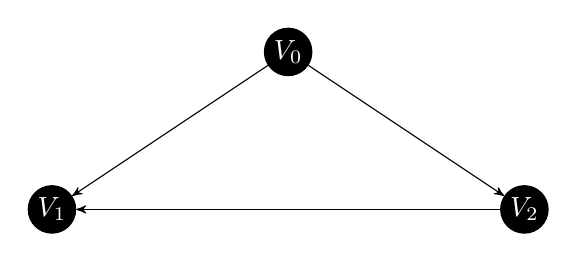
\begin{tikzpicture}[->,>=stealth',level/.style={sibling distance = 5cm/#1, level distance = 1.5cm}] 
  	[scale=.8,auto=left,every node/.style={circle}]
  	\node [arn_n] (n1) at (4,3) {$V_0$};
  	\node [arn_n] (n2) at (1,1)  {$V_1$};
  	\node [arn_n] (n3) at (7,1)  {$V_2$};

	\foreach \from/\to in {n1/n2,n1/n3,n3/n2}
    	  \draw (\from) -- (\to);
	\end{tikzpicture}
	\end{center}
	\caption{A simple directed graph with 3 nodes and 3 edges}
	\label{simple directed graph}
	\end{figure}
	

	\subsection*{Paths and Cycles}
	It is natural to consider the {\em paths} through $G$.
	A path $P$ of length $m$ is an ordered $m$-tuple of edges such that
	if the $i^{\text{th}}$ member of $P$ is an edge that points {\em to} the node $V_j$, then the $(i+1)^{\text{th}}$ member is an edge pointing {\em from} node $V_j$ {\em to} another node $V_k$ 
	(an exception obviously being the $m^{\textrm{th}}$ edge, which points to the last node along the path). 
	We refer to the first and last nodes of $P$ as the {\em starting node}, $V_s(P)$, and {\em terminal node}, $V_t(P)$, respectively. 
	 Thus, a path of length $m$ defines a sequence of $m+1$ nodes, such that each node has an edge from itself to its successor. 
	 By $\mathcal{P}(G)$, let us mean the family of all paths defined on $G$. For any $P \in \mathcal{P}(G)$, we call $P$ a {\em cycle} if $V_s(P) = V_t(P)$. We say that a graph $G$ is {\em cyclic} if there exists at least one cycle in $\mathcal{P}(G)$. Otherwise, we say that $G$ is {\em acyclic}.
	
	\subsection*{Relatives}
	The vocabulary used to describe the relationships amongst nodes in a directed graph is markedly familial. Given the nodes $V_i, V_j, V_k \in V$, we say that $V_i$ is an {\em ancestor} of $V_j$ if there exists a $P \in \mathcal{P}(G)$ such that $V_i$ precedes $V_j$ in the sequence of nodes defined by $P$. Conversely, we call $V_j$ a {\em descendant} of $V_i$. We also give special names to a node's immediate ancestors and descendants. Formally, for $V_j$, we may define the set of {\em parents} of $V_j$ as $\{V_i : (V_i,V_j) \in E \}$. Similarly, we define the set of {\em children} of $V_j$ as $\{V_k : (V_j, V_k) \in E\}$. A node whose set of parents is empty is called a {\em root} of the graph.
	
	\subsection*{The Adjacency Matrix}
	We may represent $G=(V,E)$, where $V = \{V_0, \ldots, V_{n} \}$ has order $n+1$, with an $(n+1) \times (n+1)$ matrix, $A = (a_{ij})$, such that for each entry $a_{ij}$, 
	\begin{center}
	 	$a_{ij} = 
		\begin{cases} 1, & \textrm{if\ \ \ } (V_{i-1},V_{j-1}) \in E; \\
		0, & \textrm{otherwise}. \end{cases}$
	 \end {center}
	We refer to $A$ as a {\em binary node-node adjacency matrix} or just an {\em adjacency matrix} of $G$. For example, the adjacency matrix corresponding to the first figure of this section is
	\[
	\begin{pmatrix}
	0 & 1 & 1 \\
	0 & 0 & 0 \\
	0 & 1 & 0
	\end{pmatrix} \]
	since there is an arc from $V_0$ to $V_1$, an arc from $V_0$ to $V_2$, and an arc from $V_2$ to $V_1$. We may also consider the sum of powers of $A$,
	\begin{center}
		$Y = A + A^2 + \cdots + A^{n+1} = \displaystyle\sum_{i=1}^{n+1} A^{i}$.
	\end{center}
	The resulting matrix is $(y_{ij})$, where $y_{ij}$ represents the number of unique paths $P$ where $V_s(P) \equiv V_{i-1}$, and $V_t(P) \equiv V_{j-1}$ in $\mathcal P(G)$. 
	Thus, to formalize the notion of an acyclic graph, we say that $G=(V,E)$ is acyclic if $tr(Y) = 0$. 
	Otherwise, $G$ is cyclic.
	To continue our example from above, we calculate $Y$ to be
	\[
	\begin{pmatrix}
	0 & 2 & 1 \\
	0 & 0 & 0 \\
	0 & 1 & 0
	\end{pmatrix} \]
	which is consistent with our visualization of the graph. 
	(For example, we identify two distinct paths from $V_0$ to $V_1$, so $y_{1,2} = 2$.)
	
	\section{Bayesian Networks}	
	Let $\mathcal{B} \equiv (G, \Theta)$, where $G = (V,E)$ is a directed acyclic graph, $V = \{V_0, V_1, \ldots, V_n \}$ is a set of $n + 1$ random variables, and $\Theta$ is a set of parameter estimates generated from some pre-classified data. Each parameter of $\Theta$ corresponds to an arc in the graph $G$. (That is, the parameters of our model are conditional probabilities.) We say that $\mathcal{B}$ is a Bayesian network.

	\subsection*{Restricted Bayesian Networks}
	A {\em restricted} Bayesian network caps the number of possible conditional dependencies for a given feature variable at some nonnegative integer $k$. Hence, the graph that represents the network should have at most $k$ arcs from each of its feature nodes. The Tree Augmented Network (TAN), displayed below, is an example of a restricted Bayesian Network with $k = 1$.

	\begin{figure}[htpb]
	\begin{center}
	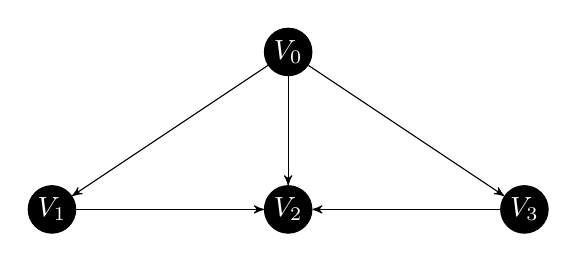
\begin{tikzpicture}[->,>=stealth',level/.style={sibling distance = 5cm/#1, level distance = 1.5cm}] 
  	[scale=.8,auto=left,every node/.style={circle,fill=blue!20}]
  	\node [arn_n] (n1) at (4,3) {$V_0$};	
  	\node [arn_n] (n2) at (1,1)  {$V_1$};
  	\node [arn_n] (n3) at (4,1)  {$V_2$};  	
	\node [arn_n] (n4) at (7,1)  {$V_3$};

	\foreach \from/\to in {n1/n2,n1/n3,n1/n4,n2/n3,n4/n3}
    	  \draw (\from) -- (\to);
	\end{tikzpicture}
	\end{center}
	\caption{TAN with three features}
	\label{simple tan}
	\end{figure}
	 Of course, a Bayesian network without restrictions on its nodes' conditional dependencies is called an {\em unrestricted} Bayesian network.
	
	\section{Bayesian Classifiers}
	A Bayesian classifier is simply a Bayesian network applied to a classification problem.
	We consider the necessary structural and decision theoretic modifications to $\mathcal{B}$ that are necessary for this application.
	
		\subsection*{Network Constraints}
	In a classification setting, we call $V_0$ the class variable, and we also place particular constraints on the graph of $\mathcal{B}$ [Liu et al, 2013].
	Namely, we require that the adjacency matrix $A$ of $G$ satisfies the following properties:
	\begin{center}
		$\displaystyle\sum_{i=1}^{n+1}a_{i1} = 0$,\ \ \ and \ \ \ 
		$\displaystyle\sum_{j=1}^{n+1}a_{1j} \neq 0$.
	\end{center}
	In words, we mean there are no directed edges pointing to the class node, and the class node has an edge to at least one feature node. Obviously, the class node is the root of $G$.
		
		\subsection*{Making a Decision}
	
	To predict the class $C$ of an input $\vec{x}$, we use a {\em decision rule}.
	Our decision rule provides a means of selecting one proposed classification over another, given a set of pre-classified data and the unclassified input $\vec{x}$.
	Recall that in surveying the general problem of classification, we chose a decision rule that returned the class maximizing our posterior probability. 
	Albeit common, this is not the only possible decision rule. 
	For instance, there may be an unequal cost associated with certain misclassifications of $\vec{x}$. In such cases, we can modify our decision rule's {\em loss function} accordingly; however, this facet of decision theory is not central to our discussion.
	 
	\subsection*{The Naive Bayes Classifier} % \"{} won't compile
	The Na\"{i}ve Bayes classifier (NBC) assumes conditional independence amongst feature variables of the model in order to yield a more wieldy computation of the posterior. 
	In light of its reductive assumption, the NBC is a surprisingly effective means of classifying data.
	
	Recall that the posterior distribution of the class variable $C \equiv X_0$ has the following property:
	\begin{center}
		$P(X_0 | X_1, \ldots , X_n) \propto
		P(X_0,\ldots,X_n) = 
		P( \displaystyle\cap_{i=0}^{n} X_i) = 
		\displaystyle\prod_{j=0}^{n} P(X_j | \displaystyle\cap_{k=0}^{j-1}X_k)$.
	\end{center}
	If we assume independence amongst the feature variables $X_1,\ldots,X_n$, then the above simplifies to
	\begin{center}
		$P(X_0) \displaystyle\prod_{j=1}^{n} P(X_j | \displaystyle\cap_{k=0}^{j-1}X_k)
		= P(C) \displaystyle\prod_{j=1}^{n} P(X_j | C)$.
	\end{center}
	Note that our independence assumption makes the NBC's graph a restricted Bayesian network with $k = 0$.
	\subsection*{Example: Spam Detection}
	Spam detection is an oft-cited example of a classification problem. It is suitable for our discussion, since it is an area of classification that has benefited greatly from application of Bayes' rule. For example, in a 1998 study, researchers at Microsoft found that existing methods for spam-filtering were significantly out-performed by a simple Na\"{i}ve Bayes classifier [Sahami et al, 1998]. We shall use their work to contextualize the preceding sections.
	
	Suppose we are given a set of 1,000 emails, and for each email, we record four pieces of information according to the table below:
	
		\begin{table}[htdp] % begins the table floating environment. This enables LaTeX to fit the table where it works best and lets you add a caption.
\caption[Example Data for Classifications]{Information on a set of 1,000 emails} 
% The words in square brackets of the caption command end up in the Table of Tables. The words in curly braces are the caption directly over the table.
\begin{center}
% makes the table centered
\begin{tabular}{| l | l |} 
 \toprule
  \textbf{Information} & \textbf{Description} \\ % the first row of the table. Separate columns with ampersands and end the line with two backslashes. An environment begun in one cell will not carry over to adjacent rows.
  \midrule % another horizontal line
   	Spam & Whether or not the email was spam \\
 	Domain & The domain of the email's sender (e.g., @reed.edu) \\	
	Hyperlinks & A count of the number of hyperlinks in the body of the email \\ % another row
  	Timestamp & The time at which the email was sent \\
\bottomrule % yet another horizontal line
\end{tabular}
\end{center}
\label{bvf} % labels are useful when you have more than one table or figure in your document. See our online documentation for more on this.
\end{table}
	Note that we assume a human has pre-classified each email as either spam or not-spam, which is necessary for our classifier to learn the parameters of the model's network.
	
	It is generally easier to learn the parameters of a Bayesian network when the feature variables are categorical. Thus, we might use the domain information to create a variable that indicates whether or not the sender's domain ended in ``.edu." For the count of hyperlinks, we might define categories of Low (0 to 4 hyperlinks), Medium (5 to 10 hyperlinks), and High (more than 10 hyperlinks). Using the timestamp of the emails, we might create an indicator for whether or not an email was sent after midnight but before 6:00 in the morning. In the end, we could assign our variables to nodes in a graph as follows:

\begin{table}[htdp] % begins the table floating environment. 
\caption[Example Training Data for Na\"{i}ve Bayes Classification]{Variables constructed from the dataset of 1,000 emails} 
% The words in square brackets of the caption command end up in the Table of Tables. The words in curly braces are the caption directly over the table.
\begin{center} 
% makes the table centered
\begin{tabular}{c | l | l} 
\toprule
  \textbf{Node} &  \textbf{Variable} & \textbf{Description}  \\ 
  \midrule % another horizontal line
 $V_0$ & spam & 1 if Spam; 0 otherwise \\ % another row
 $V_1$ & edu & 1 if from .edu; 0 otherwise \\
 $V_2$ & link-count & Low, Medium, or High \\
 $V_3$ & AM & 1 if sent between midnight and 6 am; 0 otherwise  \\
\bottomrule % yet another horizontal line
\end{tabular}
\end{center}
\label{inheritance} % labels are useful when you have more than one table or figure in your document. See our online documentation for more on this.
\end{table}
	
Because of its independence assumption, our Na\"{i}ve Bayes classifier $\mathcal B = (G,\Theta)$ has a graph with the structure depicted in Figure 1.3. To complete the classifier, we would learn our model parameters from the training set. The parameters in our example would be $P(V_0 | V_1)$, $P(V_0 | V_2)$, and $P(V_0 | V_3)$, and from the estimates of these parameters (in conjunction with the prior probabilities we would have to assign to them), it is possible to evaluate whether future incoming emails are spam.
	
	\begin{figure}[htpb]
	\begin{center}
	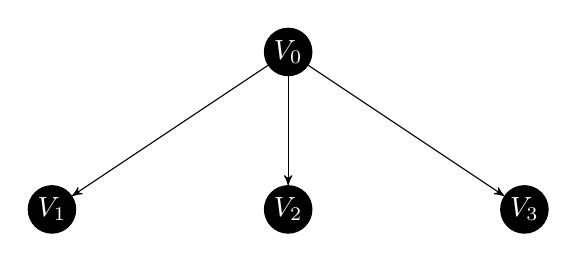
\begin{tikzpicture}[->,>=stealth',level/.style={sibling distance = 5cm/#1, level distance = 1.5cm}] 
  	[scale=.8,auto=left,every node/.style={circle,fill=blue!20}]
  	\node [arn_n] (n1) at (4,3) {$V_0$};	
  	\node [arn_n] (n2) at (1,1)  {$V_1$};
  	\node [arn_n] (n3) at (4,1)  {$V_2$};  	
	\node [arn_n] (n4) at (7,1)  {$V_3$};

	\foreach \from/\to in {n1/n2,n1/n3,n1/n4}
    	  \draw (\from) -- (\to);
	\end{tikzpicture}
	\end{center}
	\caption{A Naive Bayes Classifier} % won't compile with \"{i}
	\label{Example NBC}
	\end{figure}

	\section{Model Structure}
	We mentioned in the previous section that the Na\"{i}ve Bayes classifier is a surprisingly effective model. The performance of the NBC is surprising because in practice, feature variables are rarely independent, and ignoring the dependencies between them should give us biased probability estimates for $P(C | \vec{X})$. However, even if its probability estimates are incorrect, the NBC can still predict classifications correctly, so long as the biased estimates conform with a correct classification of the data [Domingos and Pazzani, 1996].
	
	%For example, suppose we that $C$ has two possible classes, $c_i$ and $c_j$, such that for an input $\vec{x}$, our NBC returns the biased estimates $P(c_i | \vec{x}) = .9$ and $P(c_j | \vec{x}) = .1$. Obviously, we would assign $\vec{x}$ to class $c_j$. If the unbiased estimates, obtained from a classifier that accounted for the true dependence structure of the feature variables, were $P(c_i | \vec{x}) = .6$ and $P(c_j | \vec{x})$, we would come to the same conclusion as the NBC.
	
	That being said, the NBC is not all-powerful. It works better than we would expect, but it is not guaranteed to be optimal when the feature variables of a model are not all independent of each other [Domingos and Pazzani, 1996]. Hence, to improve upon the NBC, we need a means of finding a suitable structure for a Bayesian classifier's network.
	
	\subsection*{The Structure Space}
	By $\mathcal G$, we denote the space of all possible graphs for a set of random variables, $V.$
	Unfortunately, the order of $\mathcal G$ is {\em super-exponential} on the order of $V.$ 
	Specifically, if $n$ is the number of nodes in a graph, the structure space increases in size at a rate of $2^{O(n^2\log{n})}$, which makes exhaustive search through $\mathcal G$ impractical for unrestricted networks with even a moderate number of variables [Friedman and Koeller, 2000].
	%There are ways of decreasing the size of the structure space, one of which is using restricted Bayesian networks. 

	\subsection*{Model Selection}	
		Importantly, we may choose between two modes of reasoning about model structure. 
	The first, called {\em model selection}, involves finding the most probable model structure given our data, which we can then use to estimate our parameters. Generally, this would involve cleverly searching through $\mathcal G$ (or a subset thereof) and ranking structures according to a scoring function. The structure with the highest score would be our most likely model, and we then would use it to estimate our parameters.  
	
	\subsection*{Model Averaging}
	The second technique, called {\em model averaging} is a little more nuanced. In lieu of selecting one high-scoring model, model averaging makes estimates across $\mathcal G$, which are each weighted by their probability of being the correct model. Hence, model averaging is a useful tool when we have several model structures that are roughly equiprobable. 
	
	There are a handful ways to go about model averaging, and we shall explore one of them in Chapter 2. For now, though, it suffices to know that model averaging is computationally very difficult, so we require a means to approximate it by simulation.
	
\chapter{Monte Carlo with Markov Chains}
	The reader may be familiar with Good Old Fashioned Monte Carlo (GOFMC) methods involving independent and identically distributed (IID) data. However, Monte Carlo simulations can also be done with a surprisingly simple stochastic process called a Markov chain. In fact, these Markov chain Monte Carlo (MCMC) techniques are quite useful for approximating draws from posterior distributions for which we cannot easily find the normalization constant. 
	
	This chapter provides a cursory overview of GOFMC, and then defines Markov chains with the intent of introducing a class of algorithms for Markov chain Monte Carlo simulation. 
	We close with an application of MCMC to estimating the posterior probabilities of Bayesian network structures.
	
	\section{GOFMC}
		\subsection*{An Intuitive Example}
		Imagine we seek to find the area of a peculiar two-dimensional shape called Minnesota. 
		\begin{figure}[h]
	% the options are h = here, t = top, b = bottom, p = page of figures.
	% you can add an exclamation mark to make it try harder, and multiple
	% options if you have an order of preference, e.g.
	% \begin{figure}[h!tbp]
	       	\centering
	    % DO NOT ADD A FILENAME EXTENSION TO THE GRAPHIC FILE
	    	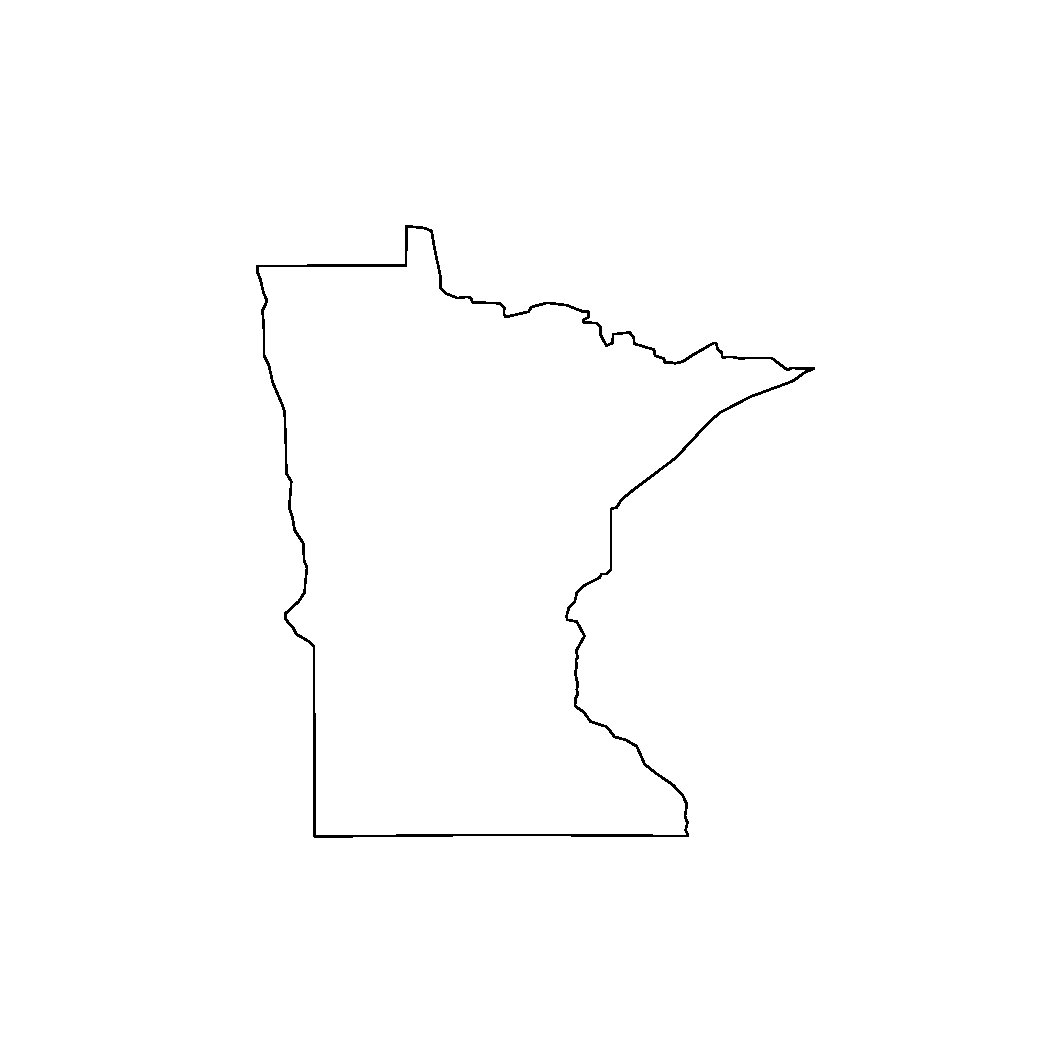
\includegraphics[clip=true, viewport=.3in 1in 6in 6in,scale=0.5]{mn}
	     	\caption{A two-dimensional shape called Minnesota}
	 	\label{subd}
		\end{figure}	
		We are given no general formula for its area, and all of our attempts to analytically represent the curve that traces its perimeter have proven themselves fruitless. With credit to a talk on Monte Carlo Tree Search given by Peter Drake at the University of Portland, the technique suggested by GOFMC would be the following:
			\begin{enumerate}
				\item Place Minnesota inside a square with edges of known length $s$.
				\item Randomly throw $n$ darts such that they land inside the square. 
				\item Record $x$, the number of darts that landed inside Minnesota.
				\item Multiply the proportion of darts that hit Minnesota ($\frac{x}{n}$) by the area of the square.
			\end{enumerate}
			Symbolically, our GOFMC estimator for the area would be
			\begin{center}
				${s^2} * \displaystyle\sum_{j=1}^{n}\frac{\iota(x_j)}{n}$,
			\end{center}
			where the $x_j$ represent dart throws, and 
			
			\begin{center}
		 	$\iota(x_j) = 
			\begin{cases} 1, & \text{if the dart hit Minnesota}; \\
			0, & \text{otherwise}. \end{cases}$
			 \end {center}
			The following illustrates our dart-throwing technique:
			
			\begin{figure}[h]
		       	\centering
		    	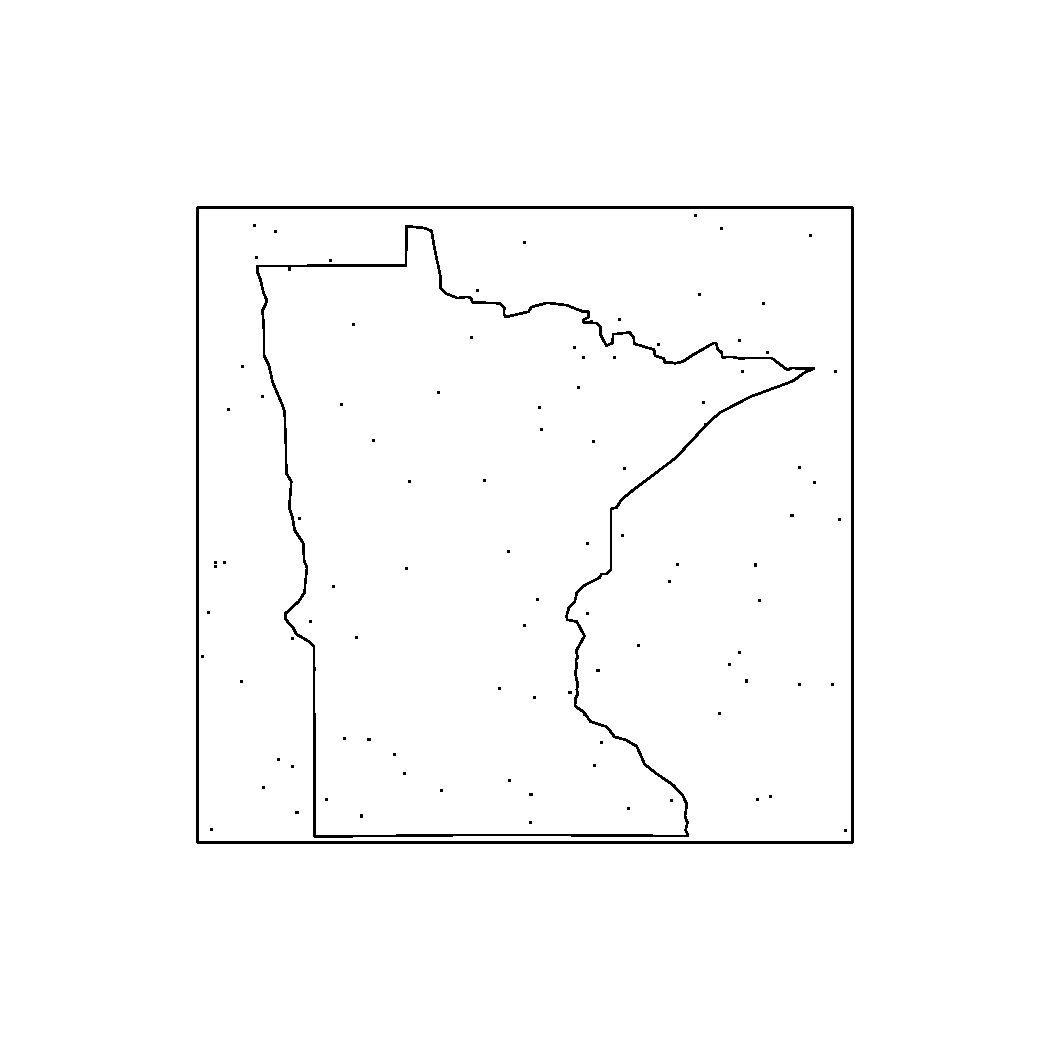
\includegraphics[clip=true, viewport=.3in 1in 6in 6in,scale=0.5]{mn_box_pts}
		     	\caption{Estimating the Area of an Oddly Shaped State}
	 		\label{subd}
			\end{figure}	

			Obviously, our estimate is not exact, but as $n \rightarrow \infty$, the Law of Large Numbers tells us that we get closer and closer to the true area of Minnesota. Thus is the motivation for GOFMC.
		\subsection*{The General Case}
			Suppose we are given a distribution $\pi$ and we seek to find the expectation of a function $f$ over $\pi$. The central idea of GOFMC is that we may generate IID random variables $X_1, \ldots, X_n$ from $\pi$ in order to estimate $E[f(\pi)]$. A logical choice of estimator would thus be
			\begin{center}
				$\displaystyle\frac{1}{n}\displaystyle\sum_{i=1}^{n}{f(X_i)}$.
			\end{center}		
			Of course, with an estimate comes the corresponding notion of its error. 
			In this case, we define the GOFMC error as
			\begin{center}
				$\epsilon = E[f(\pi)] - \displaystyle\frac{1}{n}\displaystyle\sum_{i=1}^{n}f(X_i)$.
			\end{center}
			By application of the Central Limit Theorem, we know that as $n \rightarrow \infty$, the above converges to a normal distribution with a mean $\mu = 0$ and variance inversely proportional to $n$.
			Hence, with large enough $n$, we can produce accurate estimates from our randomly generated data. 
	\section{Markov Chains}
	Andrey Markov used his eponymous chain only once in practice, to analyze the occurrence of vowels in a Pushkin poem [McGrayne, 2011]. According to legend, Enrico Fermi could run Markov chains in his head (which he did to combat insomnia), but we normal humans tend to reserve such calculations for computers [McGrayne, 2011]. Though they can be treacherous to compute, the basic intuition behind Markov chains is, thankfully, fairly easy to grasp.
	 
	 			\subsection*{Definition}
			Let $\mathcal S$ be a set of states (the {\em state space}), and let $I$ be an index set. What we call a {\em Markov chain}, denoted $\theta^{(i)}$, is a collection of states from $\mathcal S$ indexed by members of $I$, such that, for $s_j, s_k \in \mathcal S$, the probability of transitioning from some $\theta^i = s_j$ to the next state in the chain, $\theta^{i+1} = s_k$, depends solely on $s_j$, and not on any other past or future states of the chain. 
			
			Markov chains can be thought of as a sequence of probabilistic transitions from state to state.
			Thus, for any Markov chain with state space $\mathcal S$, 
			the states in $\mathcal S$ have associated {\em transition probabilities}.
			We may define a {\em transition function}, $p: \mathcal{S}\times\mathcal{S} \rightarrow [0,1],$ for a Markov chain, where $p(s_j,s_k) = P(\theta^{i+1} = s_k | \theta^{i} = s_j)$. 
			
			When $\mathcal S$ is discrete and has finite order $m$, we may specify the transition probabilities in an $m \times m$ {\em transition matrix}, $T = (t_{jk})$, where $t_{jk} = p(s_j,s_k)$. Each row of $T$ thus admits a probability distribution for a corresponding state in $\mathcal S$. 
			
			For the sake of concision, we may also refer to transitions as {\em steps}, and when the chain assumes a state $s_j$, we also say that it {\em hits} state $s_j$. 
			
	 
	\subsection*{Example: Andrey the Chameleon}
	To illustrate our definition of a Markov chain, we introduce a charismatic chameleon named Andrey. 
	Suppose that Andrey the chameleon can only assume four distinct colors: blue, green, yellow, or red. Hence, Andrey's state space $\mathcal S$ may be written as $\mathcal{S} = \{B, G, Y, R\}$. 
	
	We assume that Andrey has no control over the color to which he changes. Instead, his color changes are a probabilistic process, and each change depends only upon the color that he currently assumes. Andrey's transition matrix $T$ is given by
$$
\bordermatrix{ ~ & B & G & Y & R \cr
	                     B & .25 & .25 & .25 & .25 \cr
	                     G & .8 & .1 & .1 & 0 \cr
	                     Y & .5 & .3 & .02 & .18 \cr
	                     R & 1 & 0 & 0 & 0 \cr	                     	                     	                     
}
$$
	
	For example, $t_{2j}$ is the probability distribution $P(\theta^{i+1} | \theta^i = G)$. That is, if Andrey is currently green, he has an 80\% chance of next turning blue, a 10\% chance of remaining green, a 10\% chance of turning yellow, and a 0\% chance of turning red. 
	
	A possible run of Andrey's associated Markov chain for $1 \leq i \leq 3$ might look like the following:
	\begin{center}
		($\theta^{1} = \textrm{B},\ \  \theta^{2} = \textrm{G},\ \ \theta^{3} = \textrm{B}$).
	\end{center}
	Notice, however, that it would be impossible to observe the following collection of states:
	\begin{center}
		($\theta^{1} = \textrm{B},\ \ \theta^{2} = \textrm{R},\ \  \theta^{3} = \textrm{Y}$),
	\end{center}
	since $p(\textrm{R}, \textrm{Y}) = 0$.
	%Thus, a Markov chain is a series of states, where each state probabilistically transitions to the next state. Most importantly, the transitions only depend on the current state. It thus might help to think of the chain as a stochastic goldfish. I.e., since goldfish are notorious amnesiacs, we can imagine a scenario in which one might swim to the corner of its fishbowl, only to suddenly forget its ultimate trajectory. Hence, all that our forgetful goldfish would know is its current location. Based off of that information, it could stay put, or it could continue moving to another part of the bowl. Once we have a probabilistic description of the goldfish's next move given any position in the tank, we may define a Markov chain.
	%Andrei Markov's first application of his eponymous idea (Markov chains) was to a poem by Poeshkin. Over the next century, others found a wealth of uses for Markov chains. One recent example would be Google, whose idea of a "random surfer" informed their page ranking algorithm [cite the paper!].

		\subsection*{Basic Properties}
		We say a state $s_j \in \mathcal{S}$ is {\em irreducible} if it is possible to get to any other $s_k \in \mathcal{S}$, starting from $s_j$, in a finite number of steps. If all $s_j \in \mathcal{S}$ are irreducible, the Markov chain $\theta^{(i)}$ over $\mathcal{S}$ is also said to be irreducible. \\
		
		By $Z_j$ we denote the number of steps before a chain hits state $s_j$ for the first time. 
		We refer to this quantity as the {\em recurrence} or {\em hitting time} for state $s_j$.
		We denote the number of steps before a chain hits $s_j$ a total of $q$ times as $Z^{q}_j$, where $q \in \mathbb Z^+$. Clearly, $Z_j$ is simply shorthand for $Z^{1}_j$. We also define $Z^{0}_j = 0$. \\
		
		Since Markov chains are stochastic processes, $Z^{q}_j$ is a random variable. Hence, we may consider its expectation $E[Z^{q}_j]$. If for all $s_j \in \mathcal S$, the expected hitting time is finite ($E[Z^{1}_j] < \infty$), then we say our Markov chain is {\em positive recurrent}. \\
		
		A state $s_j$ is {\em periodic} if $\theta^{(i)}$ can only return to $s_j$ after a number of steps equal to a multiple of some positive integer $k > 1$. Markov chains that contain no periodic states are called {\em aperiodic}. We say a Markov chain is $ergodic$ if it is both aperiodic and positive recurrent. \\
		
		Lastly, the {\em stationary distribution} $\pi$ of a Markov chain is a PDF such that the transition matrix $T$ of $\theta^{(i)}$ maintains $\pi$. Symbolically, this looks like the following:
		\begin{center}
			$\displaystyle\sum_{s_j \in \mathcal S} \pi(s_j) * p(s_j,s_k) 
			= \displaystyle\sum_{s_j \in \mathcal S} \pi(s_j) * P(s_k | s_j)
			= \pi(s_k)$.
		\end{center}
		That is to say, once the run of a Markov chain enters a stationary distribution $\pi$, it stays in $\pi$.
		
%		\subsection*{An Important, Non-trivial Property}
		%An irreducible Markov chain with a finite state space $\mathcal S$ is positive recurrent. \\
%		For a stationary distribution $\pi$, we find that $\pi(s_j) * E[Z_j] = 1$. 
		
		\section{The Ergodic Theorem}
		The Ergodic Theorem for Markov chains is an analog of the Law of Large Numbers for IID data. It ties together the concepts of aperiodicity, positive recurrence, and the stationary distribution. Importantly, it is through a basic corollary to the Ergodic theorem that we are able to justify use of MCMC in order to estimate draws from intractable distributions.
		\subsection*{Preliminary Results}
		Proof of the Ergodic Theorem for Markov chains requires some preliminary results, which we provide here sans complete proofs.
		
		First, the proportion of times we hit $s_j$ in an ergodic Markov chain $\theta^{(i)}$ is the same regardless of the initial state $\theta^0$ of the chain as $n$ goes to $\infty$.
		
		Second, we define $U_{j}^q = Z_{j}^{q} - Z_{j}^{q-1}$. 
		Intuitively, this is the number of steps from the  $(q-1)^{\textrm{th}}$ hit of $s_j$ to the $q^{th}$ hit of $s_j$ in a Markov chain. 
		Clearly, then,
		\begin{center}
		 $\displaystyle\sum_{k=1}^{q}U_j^k 
		 = (Z_j^1 - Z_j^0) + \cdots + (Z_j^{q-1} - Z_j^{q-2}) + (Z_j^q - Z_j^{q-1}) 
		 = Z_j^r$. 
		 \end{center}
		 Moreover, if we consider the expectation of these quantities, we see that for all $q > 0$,
		\begin{center}
		$E[U_{j}^q] = E[Z_j^{q} - Z_j^{q-1}] = q*E[Z_j] - (q-1) *E[Z_j] = E[Z_j]$, 
		\end{center}
		This follows from the linearity of expectation.
		
		Lastly, we note that for a stationary distribution $\pi$, we have $\pi(s_j)*E[Z_j] = 1$.
		
		Rigorous treatment of the foregoing results can be found in Chapter 1 of James Norris' {\em Markov Chains} [Norris, 1998]. 
		\subsection*{Statement and Proof}
		\begin{theorem}
		Let $\theta^{(i)}$ be an ergodic Markov chain. 
		Let $V_j(n)$ be defined as follows:
		\begin{center}
			$V_j(n) = \displaystyle\sum_{i=0}^{n-1} \iota_j(\theta^{i})$,
		\end{center}
		where
		\begin{center}
			$\iota_j(\theta^i) = \begin{cases} 
				1, & \textrm{if\ \ \ } \theta^i = s_j; \\
				0, & \textrm{otherwise}. 
				\end{cases}
			$
		\end{center}
		We interpret $V_j(n)$ as the number of visits to state $s_j$ before $\theta^n$ in the Markov chain. 
		Let $E[Z_j] = m_j$ be the expected hitting time of state $s_j$. Then,
		\begin{center}
			$P\left(\displaystyle\frac{V_j(n)}{n} \longrightarrow \frac{1}{m_j}
			\textrm{, as } n \rightarrow \infty \right) = 1$.
		\end{center}
		
		That is, the proportion of times we hit $s_j$ converges in probability to the inverse of the expected recurrence time.
		\end{theorem}
		
		\begin{proof}
		Since the proportion of times we hit $s_j$ in an ergodic Markov chain is the same regardless of $\theta^0$ as $n \rightarrow \infty$, we assume without loss of generality that $s_j$ is the initial state of the chain ($\theta^0 = s_j$).
		
		Now, recall from the preliminary results that 
		\begin{center}
		 $\displaystyle\sum_{k=1}^{q}U_j^k 
		 = Z_j^q$,
		 \end{center}
		 and for all positive integers $q$, 
		 \begin{center}
			 $E[U_{j}^q] = E[Z_j] = m_j$.
		 \end{center}
		Hence, we treat $\frac{1}{n}\sum_{k=1}^{n}U_j^k$ as an estimator for $m_j$, 
		and by the Strong Law of Large Numbers, we obtain the following as $n \rightarrow \infty$: 
		\begin{center}
		$
		P\left(\displaystyle\frac{\sum_{k=1}^{n}U_j^k}{n} \rightarrow m_j \right) = 1.
		$
		\end{center}
		Now, we write
		\begin{center}
		$\displaystyle\sum_{k=1}^{V_j(n) - 1}U_j^k \leq n -1$, 
		\end{center}
		where the summation represents the number of steps until the penultimate hit of $s_j$ before $\theta^n$ in the chain.
		Obviously, then, the sum could not exceed $n -1$, since we are only considering the number of steps to a state that necessarily occurs before $\theta^{n-1}$. We may also consider 
		\begin{center}
		$\displaystyle\sum_{k=1}^{V_j(n) + 1}U_j^k \geq n$,
		\end{center}
		which is the number of steps until the first hit of $s_j$ after step $\theta^{n-1}$. 
		Thus, we may squeeze $n$ and divide the resulting inequality by $V_j(n)$, as follows:
		\begin{center}
		$$\displaystyle\frac{\displaystyle\sum_{k=1}^{V_j(n)-1}U_j^k}{V_j(n)} \leq 
		\frac{n}{V_j(n)} \leq 
		\frac{\displaystyle\sum_{k=1}^{V_j(n) + 1}U_j^k}{V_j(n)}$$.
		\end{center}
		Using the convergence of the $U_j^k$ to $m_j$, the sums become
		\begin{center}
		$$\displaystyle\frac{(V_j(n) - 1) * m_j}{V_j(n)} \leq 
		\frac{n}{V_j(n)} \leq 
		\frac{(V_j(n) + 1) * m_j}{V_j(n)}$$,
		\end{center}		
		and since $\displaystyle\lim_{n \rightarrow \infty}\frac{V_j(n) - 1}{V_j(n)} = \displaystyle\lim_{n \rightarrow \infty}\frac{V_j(n) + 1}{V_j(n)} = 1$, the above becomes
		 \begin{center}
		 	$ m_j \leq \displaystyle\frac{n}{V_j(n)} \leq m_j$.
		 \end{center}
		 Hence, as $n \rightarrow \infty$,
		 \begin{center}
		 $$
		 P\left( \displaystyle\frac{n}{V_j(n)} \longrightarrow {m_j} \right) = 1,
		 $$
		 \end{center}
		 and we have the result.
		 \end{proof}
		\subsection*{Corollary}
%		Given a bounded function $f: \mathcal{S} \rightarrow B$,
%		\begin{center}
%			$P\left( \displaystyle \frac{1}{n} \sum_{j=0}^{n-1} f(\theta^{j}) 
%			= \sum_{s_k \in \mathcal S} \pi(s_k) f(s_k) \right) = 1$, as $n \longrightarrow \infty$.
%		\end{center}
		Suppose we run an ergodic Markov chain $\theta^{(i)}$ with stationary distribution $\pi$ for $n$ steps, where $n$ is large. A consequence of the Ergodic theorem for Markov chains is that $\frac{V_j(n)}{n}$ yields an estimate of $\frac{1}{m_j}$, which is equal to $\pi(s_j)$, since $\pi(s_j) * m_j = 1$.
	\section{Metropolis-Hastings}
			Metropolis-Hastings is a class of algorithms for Markov chain Monte Carlo simulation that are particularly useful for Bayesian inference. The reason for said usefulness is that simulating draws from a posterior distribution with a Metropolis-Hastings algorithm does not require calculation of the normalization constant of the posterior. Hence, let $\pi$ be the posterior distribution, and we seek a Markov chain whose unique stationary distribution is $\pi$.
			
%			Recall that in the case of GOFMC, we have a distribution $\pi$ from which we can easily simulate random draws, and we then estimate the expectation of a function over $\pi$ through random draws from $\pi$. Thus, to perform GOFMC, we must be able to specify the distribution of $\pi$. Sometimes, however, we are not so lucky as to be able to fully compute the PDF of our distribution of interest. This occurs frequently in high-dimensional Bayesian analyses, where the denominator of our posterior calculation can be a function integrated or summed over an extremely large number of dimensions. Thus, we seek an alternative way to simulate draws from $\pi$ when we only wish to calculate the marginal of $\pi$. For this, we use a Markov chain.
			
		\subsection*{Detailed Balance}
			To construct a Markov chain $\theta^{(i)}$ with a stationary distribution equal to $\pi$, 
			we need to ensure that a stationary distribution of the chain exists. 
			To that end, given a transition function $p$, we introduce the {\em detailed balance} condition. 
			That is, for all $s_j, s_k \in \mathcal S$,
			\begin{center}
				$ \pi(s_j) p(s_j,s_k) = \pi(s_k) p(s_k,s_j)$.
			\end{center}
			It is easy to see from the definition of a stationary distribution why detailed balance guarantees the stationary distribution of $\theta^{(i)}$ exists and is equal to $\pi$. 
			We may also rearrange the detailed balance condition as follows:
			\begin{center}
				$\displaystyle \frac{\pi(s_j)}{\pi(s_k)} = \frac{p(s_k, s_j)}{p(s_j, s_k)}$.
			\end{center}
			Detailed balance is not necessary for the convergence of the chain to the posterior, but it suffices [Gamerman and Lopes, 2006]. 
		\subsection*{Proposal and Acceptance}
			Next, we consider the specifics of the transition function $p$, which must guarantee that $\pi$ is the unique stationary distribution of $\theta^{(i)}$.
			To that end, we split $p$ into a {\em proposal}, which randomly proposes a new state $S^{'} \in\mathcal S$ given the current state $S$, and an {\em acceptance rule}, $\alpha$, which returns the probability that we accept the proposed transition:
			\begin{center}
				$p(s_j,s_k) = q(s_j,s_k) \alpha(s_j,s_k)$.
			\end{center}
			We may assume the proposal is a random walk with symmetric error, and we let $q(s_j,s_k)$ be the probability $P(q(s_j) = s_k)$.
			It is not wholly necessary to require that $q$ have symmetric error, but it suffices. [Gamerman and Lopes, 2006].
			
			Construction of the acceptance rule is slightly more involved. 
			Suppose we are in state $s_j$, and $q$ proposes a move to state $s_k$. 
			We accept the transition to state $s_j$ with probability equal to
			\begin{center}
			$ \alpha(s_j,s_k) = 
			\begin{cases} \textrm{min}\{1, \frac{\pi(s_k)q(s_k, s_j)}{\pi(s_j)q(s_j, s_k)}\}, & \textrm{if\ \ \ } s_j \neq s_k; \\
			1 - \int q(s_j,s_k)\alpha(s_j,s_k)ds_k, & \textrm{otherwise}. \end{cases}
			$
			\end{center}
			When the state space $\mathcal S$ is finite, the integral above is a summation.
			
			We note that the foregoing construction of $p$ conforms with the detailed balance condition, since the symmetric error of the random walk $q$ implies $q(s_j,s_k) = q(s_k,s_j)$.
	
		\subsection*{Statement of the Algorithm}
			We choose a positive integer $N$, 
			which shall be the number of steps in the Markov chain generated by the algorithm.
			Given $N$, we proceed as follows:
			\begin{enumerate}
				\item Initialize the chain with a random state $s_j \in \mathcal S$, and record $s_j$.
				\item Propose a new state: $q(s_j) = s_k$.
				\item Accept state $s_k$ with the probability given by $\alpha(s_j,s_k)$. 
				\item Record the state to which the chain transitions in step 3.
				\item Repeat steps 2 through 4 until $N$ states have been recorded.
			\end{enumerate}
			The result is a Markov chain that, with large enough $N$, 
			converges to $\pi$, the posterior distribution.
		\subsection*{Practical Issues}
			We face two hurdles when running a Markov chain to approximate draws from the posterior. 
			First, if we sample from the chain directly, each sample depends upon the previous sample. 
			Hence, taking all of the values from our simulation would not be an IID sample from the posterior. 
			Secondly, the Markov chain may be guaranteed to converge to the posterior, but in its early iterations, the samples that it produces might not approximate the posterior distribution. 
			
			The solutions to these issues are heuristic, but they help to reduce the error of estimates made from the MCMC samples. 
			To deal with the latter issue, we can run a {\em burn-in} period for the chain, which gives the chain time to {\em mix} (enter the stationary distribution). 
			To resolve the former issue, we may employ {\em batch sampling}, which takes every $r^{\text{th}}$ state of the chain to reduce the dependence between samples.
			Although these are not perfect solutions, they tend to improve the results of MCMC in practice [Gelman et al., 2004].
			
	\section{MCMC for Bayesian Networks}
	Recall that the space of all possible networks for a Bayesian classifier is super-exponential on the number of nodes in the classifier's graph. 
	MCMC provides a practical means to reason about the posterior distribution of possible directed acyclic graphs for a Bayesian network, since the amount of computation required to find the normalization constant of the posterior is extremely intensive for even moderately-sized networks. 
	In this scenario, we consider $\mathcal G$, the space of all possible graph structures for a Bayesian network $\mathcal B$.
		\subsection*{Being Bayesian About Structure}
			Let $G \in \mathcal G$ be a possible structure for $\mathcal B$. 
			Let $D$ be the set of all observed data used to train the parameters $\Theta$ corresponding to $G$. 
			As Bayesians, we treat $G$ as a random variable, and we express the posterior of $G$ as
			\begin{center}
				$P(G | D) = \displaystyle \frac{P(D|G)P(G)}{P(D)}$,
			\end{center}
			where $P(D | G)$ is the likelihood of the data given a graph structure,
			$P(G)$ is the prior distribution on graph structures in $\mathcal G$, and
			the denominator evaluates to
			\begin{center}
				$P(D) = \displaystyle \sum_{G \in \mathcal G}P(D | G) P(G)$.
			\end{center}
			As mentioned, $P(D)$ requires a super-exponential number of computations with respect to the order of $V,$ the number of variables in the model.
			Thus, calculating the normalization constant of the posterior is undesirable. 
			However, the likelihood function for the data $D$ given a network structure $G$ has a manageable closed form expression when we the data are composed of categorical random variables [Baesans et al, 2002]. 
			If we assume that all random variables in $D$ are categorical, we can use a Metropolis-Hastings algorithm to generate samples from the posterior $P(G | D)$.
		\subsection*{The Proposal}
			Suppose the current state of the chain is $G=(V,E)$. 
			The proposal $q(G)$ for our Metropolis-Hastings algorithm randomly chooses an ordered pair of vertices $(V_i, V_j)$ for $V_i, V_j \in V, \ i \neq j$. 
			Then, if $(V_i, V_j) \in E$, $q(G)$ proposes the structure $G^{'} = (V,E - \{(V_i,V_j)\})$, which is the removal of the given arc from $E$. 
			Otherwise, if $(V_i,V_j) \not\in E$, then $q(G)$ proposes $G^{'} = (V, E \cup \{(V_i, V_j)\})$, which is the addition of the arc $(V_i, V_j)$ to $E$. Of course, such an addition must preserve the acyclic property of the graph structure. 
			We denote the count of all directed acyclic graphs with one fewer or one greater arc than $G$ as $\eta(G)$. 
			We suppose $q$ has uniform error, which implies 
			\begin{center}
			$q(G,G^{i}) = P(q(G) = G^{'}) = \frac{1}{\eta(G)}$.
			\end{center}
		\subsection*{Acceptance}
			Letting $\pi(G) = P(G|D)$,
			the acceptance rule stipulated by Metropolis-Hastings follows immediately. 
			Given the current state $G$ and the proposed structure $G^{'}$, 
			we transition to $G^{'}$ with probability equal to
			\begin{center}
				$
				\alpha(G,G^{'}) = 
				\displaystyle \min \left\{ 1, \frac{q(G^{'}, G)\pi(G^{'})}{q(G, G^{'})\pi(G)}  \right\}
				$,
			\end{center}
				which expands to
			\begin{center}
				$
				\displaystyle \min \left\{ 1, \frac{\frac{1}{\eta(G^{'})}P(G^{'} | D)P(G^{'})}{\frac{1}{\eta(G)}P(G|D)P(G)} \right\} =
				\displaystyle \min \left\{ 1, \frac{\eta(G)P(G^{'} | D)P(G^{'})}{\eta(G^{'})P(G|D)P(G)} \right\}				
				$.
			\end{center}
			Hence, running the chain according to $p$ avoids the summation over $\mathcal G$ involved in computing the normalization constant, $P(D)$.
		\subsection*{Implications for Model Selection and Model Averaging}
			By the Ergodic theorem, the posterior probability $\pi(G)$ for a graph structure can be approximated by the proportion of times that we hit the network $G$ in a run of the Metropolis-Hastings algorithm. If Metropolis-Hastings suggests that there is one structure $G$ with significantly higher posterior probability than any other $G^{'} \in \mathcal G$, we may prefer to select $G$ as the structure for our Bayesian network. However, MCMC may also reveal a suite of likely structures with roughly equal posterior probabilities. In that case, we could go the route suggested by model averaging. That is, we would make inferences while taking into account the answers provided by all structures in $\mathcal G$, weighted by their respective probabilities.
		\section{Conclusion: ``To Bayes" Continued}
			Recall from Chapter 1 the issues faced by the Na\"{i}ve Bayes Classifier. Namely, the NBC encountered biases because it failed to accurately represent the conditional dependencies between its feature variables. 
			We concluded that in order to build an optimal classifier, we would need a means to find a good model structure, given the data. 
			However, when the number of nodes in $G$ was even moderately large, applying Bayes' theorem to $P(G | D)$ returned a posterior distribution with an unwieldily normalization constant. 
			
			Ultimately, we found that, under certain conditions, Monte Carlo simulation with a Markov chain that converged to the posterior $P(G | D)$ could be used by means of a simple Metropolis-Hastings algorithm to help find the most probable graph structure(s) for a Bayesian network $\mathcal{B}$. 
			The Metropolis-Hastings algorithm that we described avoided the computation of the normalization constant of $P(G | D)$, and thus would allow us to make a statement about the probability of correctness for a specific Bayesian network given the data and the prior distribution on network structures.
			
			
									
%\chapter{Bayesian Model Averaging for Bayesian Networks}
%	\section{Bayes' Theorem for Models}
%	\section{MCMC for BMA}
%If you feel it necessary to include an appendix, it goes here.
%   \appendix
%      \chapter{Appendix A}
%       \section{The Chain Rule for Probability}


%This is where endnotes are supposed to go, if you have them.
%I have no idea how endnotes work with LaTeX.

  \backmatter % backmatter makes the index and bibliography appear properly in the t.o.c...

\newpage
\begin{thebibliography}{1}

\bibitem{baes} B. Baesens, M. Egmont-Petersen, R. Castelo, and J. Vanthienen. Learning Bayesian network classifiers for credit scoring using Markov Chain Monte Carlo search. {\em Proceedings of the 16th International Conference on Pattern Recognition}, 2002. doi: 10.1109/ICPR.2002.1047792

\bibitem{domi} P. Domingos and M. Pazzani. Beyond Independence: Conditions for the Optimality of the Simple Bayesian Classifier. {\em Proceedings of the International Conference on Machine Learning}, 1996. URL https://www.ics.uci.edu/~pazzani/Publications/mlc96-pedro.pdf

\bibitem{kiel} N. Friedman and D. Koller. Being Bayesian About Network Structure. Netherlands: Kluwer Academic Publishers, 2000. URL http://robotics.stanford.edu/~koller/Papers/Friedman+Koller:MLJ03.pdf

\bibitem{mcmc} D. Gamerman and H. F. Lopes. {\em Markov Chain Monte Carlo}. Boca Raton, FL: Chapman \& Hall/CRC, 2006.

\bibitem{gelm} A. Gelman, J. B. Carlin, H. S. Stern, and D. B. Rubin. {\em Bayesian Data Analysis}, 2nd ed. Boca Raton, FL: Chapman \& Hall/CRC, 2004.

\bibitem{heck} D. Heckerman. A Tutorial on Learning With Bayesian Networks. Microsoft Research, 1995. URL https://research.microsoft.com/pubs/69588/tr-95-06.pdf

\bibitem{liu} S. Liu, M. Zhu, and Y. Yang. A Bayesian Classifier Learning Algorithm Based on Optimization Model. {\em Mathematical Problems in Engineering}, 2013. doi: 10.1155/2013/975935 % wtf is DOI?

\bibitem{hist} S.B. McGrayne. {\em The theory that would not die: How Bayes' rule cracked the enigma code, hunted down Russian submarines, and emerged triumphant from two centuries of controversy}. New Haven, CT: Yale University Press, 2011.

\bibitem{norr} J. R. Norris. {\em Markov Chains}. Cambridge, UK: Cambridge University Press, 1998. ISBN 0521633966

\bibitem{msft} M. Sahami, S. Dumais, D. Heckerman, and E. Horvitz. A Bayesian approach to filtering junk email., AAAI Workshop on Learning for Text Categorization, July 1998, Madison, Wisconsin. AAAI Technical Report WS-98-05.

\end{thebibliography}
% if you're using bibtex, the next line forces every entry in the bibtex file to be included
% in your bibliography, regardless of whether or not you've cited it in the thesis.
%%%    \nocite{*}

% Rename my bibliography to be called "Works Cited" and not "References" or ``Bibliography''
% \renewcommand{\bibname}{Works Cited}

%    \bibliographystyle{bsts/mla-good} % there are a variety of styles available; 
%  \bibliographystyle{plainnat}
% replace ``plainnat'' with the style of choice. You can refer to files in the bsts or APA 
% subfolder, e.g. 
 %%%\bibliographystyle{APA/apa-good}  % or
 %%%\bibliography{thesis}
 % Comment the above two lines and uncomment the next line to use biblatex-chicago.
 %\printbibliography[heading=bibintoc]

% Finally, an index would go here... but it is also optional.
\end{document}
